\documentclass[12pt]{article}

\usepackage{amsmath, mathtools}
\usepackage{amsfonts}
\usepackage{amssymb}
\usepackage{graphicx}
\usepackage{colortbl}
\usepackage{xr}
\usepackage{hyperref}
\usepackage{longtable}
\usepackage{xfrac}
\usepackage{tabularx}
\usepackage{float}
\usepackage{siunitx}
\usepackage{booktabs}
\usepackage{caption}
\usepackage{pdflscape}
\usepackage{afterpage}
\usepackage{placeins}
\usepackage[shortlabels]{enumitem}

\usepackage[round]{natbib}

%\usepackage{refcheck}

\hypersetup{
    bookmarks=true,         % show bookmarks bar?
    colorlinks=true,        % false: boxed links; true: colored links
    linkcolor=red,          % color of internal links (change box color with linkbordercolor)
    citecolor=green,        % color of links to bibliography
    filecolor=magenta,      % color of file links
    urlcolor=cyan           % color of external links
}

%% Comments

\usepackage{color}

\newif\ifcomments\commentstrue %displays comments
%\newif\ifcomments\commentsfalse %so that comments do not display

\ifcomments
\newcommand{\authornote}[3]{\textcolor{#1}{[#3 ---#2]}}
\newcommand{\todo}[1]{\textcolor{red}{[TODO: #1]}}
\else
\newcommand{\authornote}[3]{}
\newcommand{\todo}[1]{}
\fi

\newcommand{\wss}[1]{\authornote{blue}{SS}{#1}} 
\newcommand{\plt}[1]{\authornote{magenta}{TPLT}{#1}} %For explanation of the template
\newcommand{\an}[1]{\authornote{cyan}{Author}{#1}}

%% Common Parts

\newcommand{\progname}{Sayyara}
\newcommand{\authname}{Team 3, Tiny Coders
	\\ Arkin Modi
	\\ Joy Xiao
	\\ Leon So
	\\ Timothy Choy} % AUTHOR NAMES

\usepackage{hyperref}
\hypersetup{colorlinks=true, linkcolor=blue, citecolor=blue, filecolor=blue,
	urlcolor=blue, unicode=false}
\urlstyle{same}

\usepackage{parskip}
\usepackage{geometry}
\geometry{a4paper, portrait, margin=1in}


% For easy change of table widths
\newcommand{\colZwidth}{1.0\textwidth}
\newcommand{\colAwidth}{0.13\textwidth}
\newcommand{\colBwidth}{0.82\textwidth}
\newcommand{\colCwidth}{0.1\textwidth}
\newcommand{\colDwidth}{0.05\textwidth}
\newcommand{\colEwidth}{0.8\textwidth}
\newcommand{\colFwidth}{0.17\textwidth}
\newcommand{\colGwidth}{0.5\textwidth}
\newcommand{\colHwidth}{0.28\textwidth}

% Used so that cross-references have a meaningful prefix
\newcounter{defnum} %Definition Number
\newcommand{\dthedefnum}{GD\thedefnum}
\newcommand{\dref}[1]{GD\ref{#1}}
\newcounter{datadefnum} %Datadefinition Number
\newcommand{\ddthedatadefnum}{DD\thedatadefnum}
\newcommand{\ddref}[1]{DD\ref{#1}}
\newcounter{theorynum} %Theory Number
\newcommand{\tthetheorynum}{TM\thetheorynum}
\newcommand{\tref}[1]{TM\ref{#1}}
\newcounter{tablenum} %Table Number
\newcommand{\tbthetablenum}{TB\thetablenum}
\newcommand{\tbref}[1]{TB\ref{#1}}
\newcounter{assumpnum} %Assumption Number
\newcommand{\atheassumpnum}{A\theassumpnum}
\newcommand{\aref}[1]{A\ref{#1}}
\newcounter{goalnum} %Goal Number
\newcommand{\gthegoalnum}{GS\thegoalnum}
\newcommand{\gsref}[1]{GS\ref{#1}}
\newcounter{instnum} %Instance Number
\newcommand{\itheinstnum}{IM\theinstnum}
\newcommand{\iref}[1]{IM\ref{#1}}
\newcounter{reqnum} %Requirement Number
\newcommand{\rthereqnum}{R\thereqnum}
\newcommand{\rref}[1]{R\ref{#1}}
\newcounter{nfrnum} %NFR Number
\newcommand{\rthenfrnum}{NFR\thenfrnum}
\newcommand{\nfrref}[1]{NFR\ref{#1}}
\newcounter{lcnum} %Likely change number
\newcommand{\lthelcnum}{LC\thelcnum}
\newcommand{\lcref}[1]{LC\ref{#1}}

\usepackage{fullpage}

\newcommand{\deftheory}[9][Not Applicable]
{
\newpage
\noindent \rule{\textwidth}{0.5mm}

\paragraph{RefName: } \textbf{#2} \phantomsection
\label{#2}

\paragraph{Label:} #3

\noindent \rule{\textwidth}{0.5mm}

\paragraph{Equation:}

#4

\paragraph{Description:}

#5

\paragraph{Notes:}

#6

\paragraph{Source:}

#7

\paragraph{Ref.\ By:}

#8

\paragraph{Preconditions for \hyperref[#2]{#2}:}
\label{#2_precond}

#9

\paragraph{Derivation for \hyperref[#2]{#2}:}
\label{#2_deriv}

#1

\noindent \rule{\textwidth}{0.5mm}

}

\begin{document}

\title{Software Requirements Specification for \progname: Progressive Web Application for Independent
	Automotive Repair Shop Industry}
\author{\authname}
\date{\today}

\maketitle

\newpage

\pagenumbering{roman}

\tableofcontents

\newpage

\listoftables

\listoffigures

\newpage

\begin{longtable}{p{0.2\textwidth} p{0.2\textwidth} p{0.5\textwidth}}
	\caption{Revision History} \label{TblRevisionHistory}                                                                           \\
	\toprule
	\textbf{Date}      & \textbf{Developer(s)} & \textbf{Change}                                                                    \\
	\midrule
	September 30, 2022 & Leon So               & Add purpose of project                                                             \\
	September 30, 2022 & Joy Xiao              & Add stakeholders                                                                   \\
	September 30, 2022 & Leon So               & Add functional requirements for authentication                                     \\
	September 30, 2022 & Arkin Modi            & Add open issues and new problems sections (effects on the current environment)     \\
	October 1, 2022    & Timothy Choy          & Add mandated constraints                                                           \\
	October 1, 2022    & Arkin Modi            & Add user documentation and training, waiting room and ideas for solutions sections \\
	October 1, 2022    & Arkin Modi            & Add project planning, migration to the new product, risks, and costs sections      \\
	October 2, 2022    & Leon So               & Add current situation and appointment diagram                                      \\
	October 2, 2022    & Joy Xiao              & Add current situation quote and invitation diagram                                 \\
	October 3, 2022    & Leon So               & Add current situation work order diagram                                           \\
	October 3, 2022    & Leon So               & Add functional requirements for employees management                               \\
	October 3, 2022    & Joy Xiao              & Add appointment FRs                                                                \\
	October 3, 2022    & Arkin Modi            & Add planning of the development phases and new problems sections                   \\
	October 3, 2022    & Arkin Modi            & Add off-the-shelf solutions sections                                               \\
	October 3, 2022    & Arkin Modi            & Add functional requirements for work orders                                        \\
	October 3, 2022    & Timothy Choy          & Add functional requirements for shop profile                                       \\
	October 4, 2022    & Timothy Choy          & Add functional requirements for employee profile                                   \\
	October 4, 2022    & Leon So               & Add context of work diagram                                                        \\
	October 4, 2022    & Leon So               & Add SRS subtitle                                                                   \\
	October 4, 2022    & Joy Xiao              & Add service functional requirements                                                \\
	October 4, 2022    & Arkin Modi            & Add functional requirements for quotes                                             \\
	October 4, 2022    & Joy Xiao              & Add non functional requirements                                                    \\
	October 5, 2022    & Leon So               & Add functional requirements for password reset                                     \\
	October 5, 2022    & Arkin Modi            & Add naming conventions and terminology section                                     \\
	October 5, 2022    & Leon So               & Add reflection in Appendix                                                         \\
	October 5, 2022    & Joy Xiao              & Add work partitioning                                                              \\
	October 5, 2022    & Leon So               & Add personas                                                                       \\
	October 5, 2022    & Timothy Choy          & Add functional requirements for shop lookup                                        \\
	October 5, 2022    & Timothy Choy          & Add individual product use cases                                                   \\
	October 5, 2022    & Timothy Choy          & Add formal specifications                                                          \\
	October 5, 2022    & Leon So               & Add relevant facts and assumptions                                                 \\
	October 5, 2022    & Arkin Modi            & Add reflection                                                                     \\
	October 5, 2022    & Leon So               & Add reflection                                                                     \\
	October 5, 2022    & Timothy Choy          & Add reflection                                                                     \\
	October 5, 2022    & Joy Xiao              & Add reflection                                                                     \\
	October 19, 2022   & Timothy Choy          & Update requirements from Hazard Analysis                                           \\
	March 4, 2023      & Timothy Choy          & Update Usability and Humanity Nonfunctional Requirements                           \\
	March 5, 2023      & Timothy Choy          & Update Performance Nonfunctional Requirement                                       \\
	March 5, 2023      & Leon So               & Remove Employee Profile requirements \& remove Shop Profile update requirements    \\
	March 6, 2023      & Leon So               & Update Functional Requirements for Authentication                                  \\
	March 6, 2023      & Leon So               & Update Functional Requirements for Employee Management                             \\
	March 6, 2023      & Timothy Choy          & Update Functional Requirements for Shop Lookup                                     \\
	March 6, 2023      & Joy Xiao              & Update services and appointments requirements                                      \\
	March 6, 2023      & Arkin Modi            & Update Functional Requirements for Quotes                                          \\
	March 6, 2023      & Leon So               & Update to remove emails for employee sign up                                       \\
	March 7, 2023      & Arkin Modi            & Update Functional Requirements for Work Orders                                     \\
	March 8, 2023      & Timothy Choy          & Update Usability Nonfunctional Requirement                                         \\
	March 8, 2023      & Joy Xiao              & Remove requirements for shop/employee to edit appointment time                     \\
	\bottomrule
\end{longtable}

\newpage

\pagenumbering{arabic}

This document describes the requirements for Sayyara. The template for the Software Requirements
Specification (SRS) is a subset of the Volere template~\citep{RobertsonAndRobertson2012}. This
template has been modified to include personas to represent different user types. It has also been
modified to add formal specifications.

\section{Project Drivers}

\subsection{The Purpose of the Project}

Independent auto repair shops do not have an efficient way of reaching and interacting with new
customers. Currently, many independent shop owners rely on word-of-mouth referrals as a main
channel to acquiring new customers. Independent auto repair shops are also spending a significant
amount of their time on administrative work such as managing appointments and providing quotes. As
a result, independent auto repair shops have a difficult time competing with larger repair shops
which have dedicated systems and services in place.

On the other hand, customers do not have an effective way to find and compare auto repair shops.
Currently, one of the only ways to compare repair shops is by manually searching or reaching out to
repair shops one-by-one. This process can often be repetitive and time-consuming.

Sayyara is a progressive web application (PWA) which will act as a single platform for independent
auto repair shops and vehicle owners. This platform will allow independent auto repair shops and
vehicle owners to interact in a more efficient and effective manner. Vehicle owners can search for
auto repair shops and services based on a variety of search filters; request quotes for service;
book, view, and manage service appointments. On the application, auto repair shop owners will have
full shop management capabilities such as: adding and managing a list of employees; managing a list
of service types and corresponding service appointment availabilities; managing store information
such as location, hours of operation, and contact information. Auto repair shop owners and
employees will be able to manage quotes, service appointments, and work orders from a single
application. Ultimately, Sayyara will significantly improve the auto repair experience for both
independent auto repair shops and vehicle owners.

\subsection{The Stakeholders}

\subsubsection{The Client}
The client of the project is Nabeel Ibrahim. Nabeel will be the point of contact throughout the
development of the project.

\subsubsection{The Customers}
The customers of Sayyara will be independent auto repair shop owners, shop employees, and vehicle
owners who are looking for a vehicle repair or maintenance service.

\subsubsection{Other Stakeholders}
Other stakeholders of the project are the developers, Tiny Coders, who are designing and
implementing the project.

\subsection{Personas}
\begin{enumerate}
	\item Albert Lee is a 25 year old professional working in the accounting industry from Markham, Ontario.
	      He has a wife and three children. Mr. Lee's family two cars: a silver 2005 Toyota Prius LE and a
	      black 2014 Honda CRV. He commutes to Vaughan, Ontario for work. On his way to work each morning, he
	      drops off his children at school. He prefers to drive the Prius for his work commute to save on
	      gas. However, on weekend road trips, grocery shopping, and driving his kids to soccer practice, he
	      prefers to drive the CRV. This is because the car is more spacious and can fit more cargo. Albert
	      has a busy schedule, but he is adamant in making sure his cars are regularly maintained. This is
	      because he believes that safety is important, and keeping his vehicles well-maintained will allow
	      his vehicles to have a longer useful-life. Albert is also very cost-conscious and likes to make
	      sure that he is getting the best value for anything he pays for.
	\item David Jones is a 60 year old independent auto repair shop owner in Hamilton, Ontario. He has been
	      operating his repair shop for over 35 years. David currently has 3 employees working for him: one
	      receptionist, and one mechanic, and one apprentice. David splits his time working on administrative
	      tasks, servicing cars, and overlooking the work of his employees. He is a very organized individual
	      and expects the same from his employees. David also believes that customer service is very
	      important, and only by providing the best value and service, can he compete with larger auto repair
	      and maintenance franchises.
	\item Alice Stark is a 22 year old Uber driver. She enjoys working for the platform due to the flexible
	      schedule. Alice drives a 2016 Chevy Cruze. On Uber, she delivers food and provides rides to
	      passengers. The service she offers depends on the time of day. During lunch and dinner hours, she
	      prefers to deliver food through Uber Eats due to the higher volume of orders. She also loves
	      interacting with people and customers, and hearing about their unique life stories. When she is not
	      working, she enjoys spending her time meeting her friends at restaurants, hiking, and playing
	      sports. Her car is very important to her, and it is an important part of her everyday. When she
	      needs auto repairs or maintenance, she likes to find high quality services which use OEM parts. She
	      does not mind paying more for quality work and parts because of how important her car is in her
	      daily life. However, since she has a very busy day and her work depends on her car, she also cares
	      about the service speed. It is important that her car can be repaired and fixed promptly.
	\item Alex Snow is a 42 year old auto repair mechanic working at a local repair shop in Burlington,
	      Ontario. Alex graduated as a mechanical engineer from the University of Waterloo 20 years ago.
	      Since graduating, he decided to dedicate his time to his passion of fixing cars. He likes to
	      maximize his time working on cars. Alex takes a lot of pride in his work, and wants to ensure that
	      each customer is satisfied with his work. Alex specializes in more advance repairs such as changing
	      transmissions, engine replacements, replacing cylinder blocks, and much more. He rarely spends time
	      on simpler services such as oil changes, brake replacement, and tire changes. These are the most
	      common repairs the shops sees, but are usually delegated to less experienced employees in the shop.
\end{enumerate}
\subsection{Mandated Constraints}

\subsubsection{Solution Constraints}
\emph{Description:} The product shall be built as a Progressive Web Application (PWA)\\
\emph{Rationale:} The supervisor wants the application to be a PWA\\
\emph{Fit Criterion:} The product shall be written using the Next.js PWA plugin

\emph{Description:} The product shall be able to function on a variety of devices, such as on a computer, on tablets and on most modern phones\\
\emph{Rationale:} Users will be accessing this product in a variety of scenarios, and will have access to different devices\\
\emph{Fit Criterion:} The product shall be tested to function properly on Chrome's device toolbar, which includes the following devices:
\begin{itemize}
	\item iPhone SE
	\item iPhone XR
	\item iPhone 12 Pro
	\item Pixel 5
	\item Samsung Galaxy S8+
	\item Samsung Galaxy S20 Ultra
	\item iPad Air
	\item iPad Mini
	\item Surface Pro 7
	\item Surface Duo
	\item Galaxy Fold
	\item Samsung Galaxy A51/71
	\item Nest Hub
	\item Nest Hub Max
\end{itemize}

However, due to timing constraints, testing will only be run on the most popular cases, which would
include the iPhone, Pixel and Samsung phones, as well as iPad and Galaxy tablets.

\subsubsection{Implementation Environment of the Current System}
In the current design of the product, the product shall be implemented in a cloud hosted serverless
environment. In this specific case, it shall be AWS Lambda. The product itself shall also be able
to function properly with any web browser and operating system.

\subsubsection{Partner or Collaborative Applications}
In the current design of the product, there are no partner or collaborative applications that will
work along with the product. Therefore, there are no partner or collaborative constraints.

\subsubsection{Off-the-Shelf Software}
The following off-the-shelf software will be utilized:
\begin{itemize}
	\item Next.js (and Next PWA)
\end{itemize}

\subsubsection{Anticipated Workplace Environment}
The anticipated workplace environment will be very broad. The product can be used from anywhere the
user has access to a device and internet to run the application.

\subsubsection{Schedule Constraints}
As stated in the SFWRENG 4G06 course outline, the schedule constraints are as follows:
\begin{table}[H]
	\centering
	\caption{Schedule Constraints}
	\vspace{5pt}
	\begin{tabular}{|p{0.3\textwidth}|p{0.6\textwidth}|}
		\hline
		\textbf{Date}   & \textbf{Deliverable}               \\
		\hline
		Oct 19, 2022    & Hazard Analysis                    \\
		\hline
		Nov 2, 2022     & Verification and Validation Plan   \\
		\hline
		Nov 14-25, 2022 & Proof of Concept Demo              \\
		\hline
		Jan 18, 2023    & Design Document                    \\
		\hline
		Feb 6-17, 2023  & Revision 0 Demo                    \\
		\hline
		Mar 8, 2023     & Verification and Validation Report \\
		\hline
		Mar 20-31, 2023 & Final Demo (Rev 1)                 \\
		\hline
		Apr 5, 2023     & Final Documentation                \\
		\hline
	\end{tabular}
\end{table}

\subsubsection{Budget Constraints}
The project has no monetary budget. If there are any necessary purchases for development, the cost
shall be paid by the project members and reimbursed by the supervisor. Furthermore, these purchases
may not exceed \$750.

\subsubsection{Enterprise Constraints}
The project will require authentication in the form of users logging in. The current implementation
of the project will require users to authenticate with a username and password. In the future, SSO
may be used.

\subsection{Naming Conventions and Terminology}
\begin{table}[H]
	\caption{Naming Conventions and Terminology}
	\centering
	\begin{tabular}{ |p{5cm}|p{10.5cm}|  }
		\hline
		\textbf{Term}                         & \textbf{Definition}                                                      \\
		\hline
		Progressive Web Application (PWA)     & Progress Web Application use web-platform features to give
		users an experience on par with native applications. These features include: being installable,
		native notification, and offline capabilities.                                                                   \\
		\hline
		Amazon Web Services (AWS)             & Amazon Web Services is a cloud computing provider.                       \\
		\hline
		Amazon Web Services (AWS) Lambda      & Amazon Web Services' serverless compute unit.                            \\
		\hline
		Chrome                                & Google Chrome is a cross-platform web browser developed by Google.       \\
		\hline
		Sayyara                               & Sayyara is the name of the company the project
		supervisor operates runs and the name of the application.                                                        \\
		\hline
		Vehicle Identification Number (VIN)   & A Vehicle Identification Number is an alphanumeric string
		containing the exact details about a car's make, model and manufacturing                                         \\
		\hline
		Original Equipment Manufacturer (OEM) & An Original Equipment Manufacturer is the original
		manufacturer of a component or product.                                                                          \\
		\hline
		Next.js                               & A React based framework.                                                 \\
		\hline
		NextAuth.js                           & A React based authentication library for Next.js.                        \\
		\hline
		React                                 & A JavaScript library for building user interfaces.                       \\
		\hline
		Node.js                               & An open-source, cross-platform, back-end JavaScript runtime environment. \\
		\hline
	\end{tabular}
\end{table}

\subsection{Relevant Facts and Assumptions}
\subsubsection{Users}
\begin{enumerate}
	\item It is assumed that users have a valid email address.
	\item It is assumed that the user will have internet connection when using the application.
	\item It is assumed that the user is located in Canada.
\end{enumerate}

\textbf{Vehicle Owners}
\begin{enumerate}
	\item It is assumed that users looking for auto repair or maintenance own at least one vehicle.
\end{enumerate}

\textbf{Auto Repair Shop Owners}
\begin{enumerate}
	\item For the initial version of Sayyara, there can only be one owner account per auto repair shop.
	\item It is assumed that the auto repair shop is located in Canada.
\end{enumerate}

\textbf{Auto Repair Shop Employees}
\begin{enumerate}
	\item It is assumed that employees are only employed at one auto repair shop.
\end{enumerate}

\subsubsection{Services}
\begin{enumerate}
	\item It is assumed that only auto repair shop owners can add and edit the list of services.
\end{enumerate}

\subsubsection{Employee Management}
\begin{enumerate}
	\item For the initial version of the application, employees can only sign up using a shop ID provided by
	      the shop owner.
	\item For the initial version of the application, only auto repair shop owners can access the shop ID.
	\item It is assumed that only the auto repair shop owner can edit and remove employees.
\end{enumerate}

\subsubsection{Other}
\begin{enumerate}
	\item For the initial version of the application, Sayyara will not process any payment transactions.
\end{enumerate}

\section{Functional Requirements}

\subsection{The Scope of the Work and the Product}

\subsubsection{The Current Situation}
The current interactions between independent auto repair shop owners, employees, and customers
(i.e., vehicle owners), are often a manual process. Outlined below are models for interactions
between the independent auto repair shop owners, employees, customers, and the proposed system.
\begin{figure}[!hbp]
	\centering
	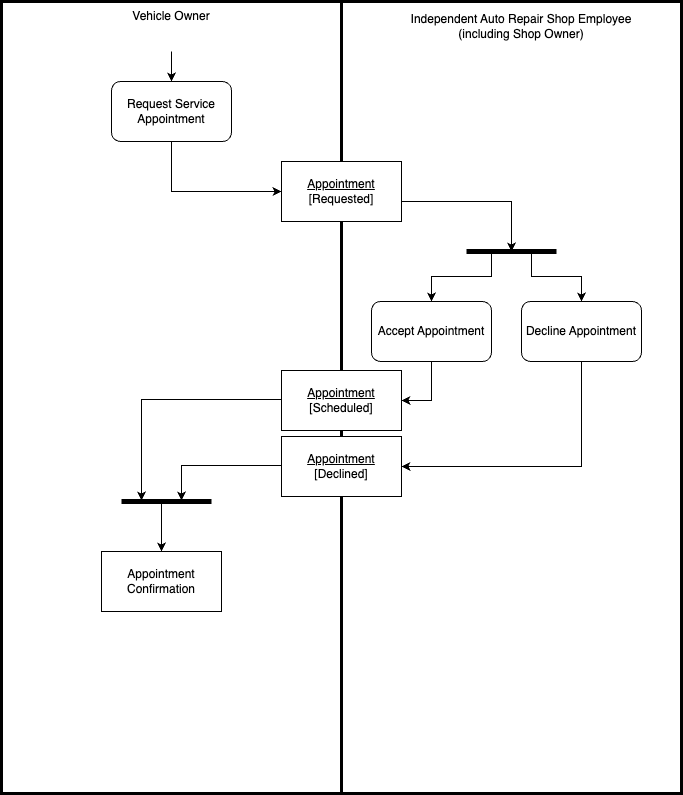
\includegraphics[width=\linewidth/2]{./diagrams/Appointments.png}
	\caption{Service Appointments}
\end{figure}
\FloatBarrier
\begin{figure}[!hbp]
	\centering
	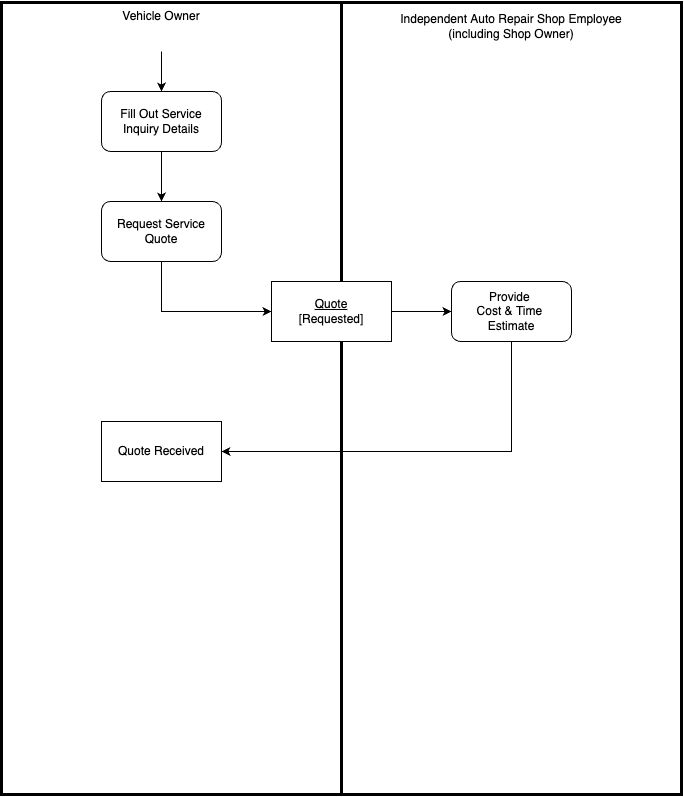
\includegraphics[width=\linewidth/2]{./diagrams/Quotes.png}
	\caption{Service Quotes}
\end{figure}
\FloatBarrier
\begin{figure}[!hbp]
	\centering
	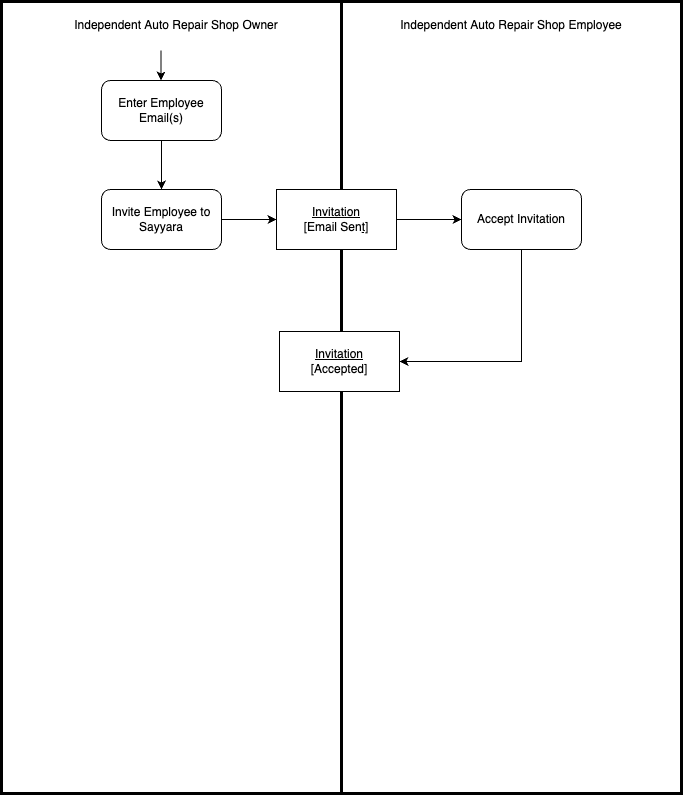
\includegraphics[width=\linewidth/2]{./diagrams/Invitation.png}
	\caption{Employee Invitation to Join Auto Repair Shop}
\end{figure}
\FloatBarrier
\begin{figure}[!hbp]
	\centering
	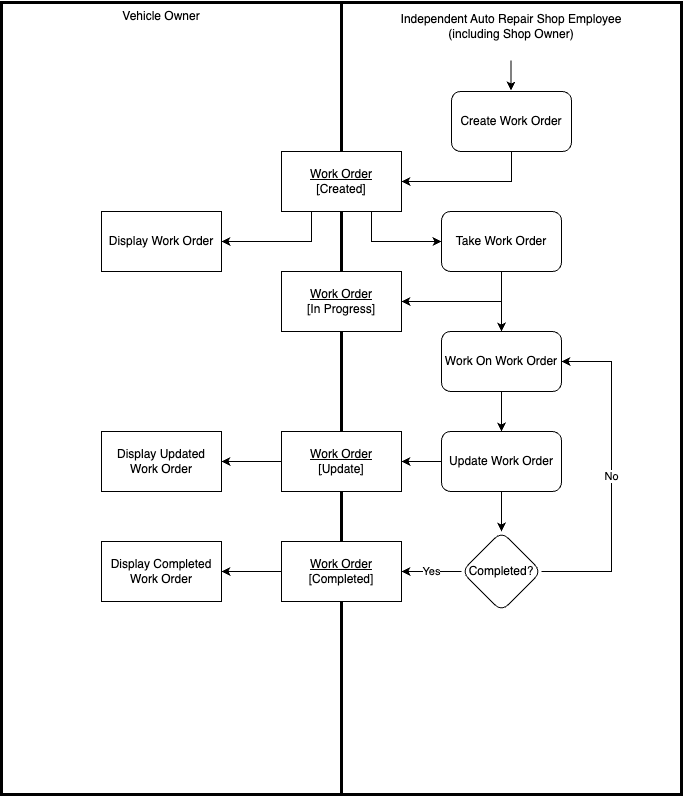
\includegraphics[width=\linewidth/2]{./diagrams/WorkOrder.png}
	\caption{Work Orders}
\end{figure}
\FloatBarrier

\subsubsection{Context of the Work}
The context diagram depicted below illustrates the interactions of the system with adjacent
external systems and services.
\begin{figure}[!hbp]
	\centering
	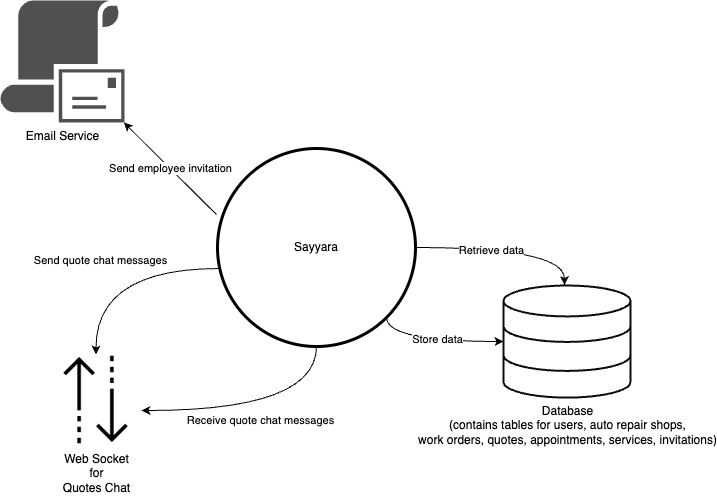
\includegraphics[width=\linewidth/2]{./diagrams/ContextOfWork.png}
	\caption{Context Diagram (Sayyara)}
\end{figure}
\FloatBarrier

\newpage
\subsubsection{Work Partitioning}
\begin{table}[H]
	\caption{Work Partitioning Events}
	\centering
	\begin{tabular}{|c|p{3.5cm}|c|p{3.5cm}|}
		\hline
		\textbf{Event Number} & \centering\textbf{Event Name}  & \textbf{Input} & \textbf{Output}    \\
		\hline
		1                     & Sign up for account            & User           & Database           \\
		\hline
		2                     & Login to account               & User           & Database           \\
		\hline
		3                     & Book appointment               & Database       & Database           \\
		\hline
		4                     & Edit appointment               & Database       & Database           \\
		\hline
		5                     & Cancel appointment             & Database       & Database           \\
		\hline
		6                     & Set appointment availability   & Database       & Database           \\
		\hline
		7                     & View past quotes               & User           & Database           \\
		\hline
		8                     & View quote details             & User           & Database           \\
		\hline
		9                     & Request a quote                & Web Socket     & Database           \\
		\hline
		10                    & Cancel quote request           & User           & Database           \\
		\hline
		11                    & Update quote request           & User           & Database/Websocket \\
		\hline
		12                    & Copy a quote request           & Database       & Database/Websocket \\
		\hline
		13                    & Respond to quote request       & Websocket      & Database           \\
		\hline
		14                    & Accept quote response          & Websocket      & Database           \\
		\hline
		15                    & Request additional information & Websocket      & Database           \\
		\hline
		16                    & Appointment scheduled          & User           & Database           \\
		\hline
		17                    & Appointment cancelled          & User           & Database           \\
		\hline
		18                    & Search for work order          & User           & Database           \\
		\hline
	\end{tabular}
\end{table}

\begin{table}[H]
	\caption{Work Partitioning Events Continued}
	\centering
	\begin{tabular}{|c|p{3.5cm}|c|p{3.5cm}|}
		\hline
		\textbf{Event Number} & \centering\textbf{Event Name}     & \textbf{Input} & \textbf{Output}        \\
		\hline
		20                    & View past work orders             & User           & Database               \\
		\hline
		21                    & Update work order                 & User           & Database               \\
		\hline
		22                    & Work order payment                & User           & Database/Email service \\
		\hline
		23                    & View work order details           & User           & Database               \\
		\hline
		24                    & Invite employee to shop           & User           & Database/Email service \\
		\hline
		25                    & Search for employee               & User           & Database               \\
		\hline
		26                    & View list of employees            & User           & Database               \\
		\hline
		27                    & Remove employee from shop         & User           & Database               \\
		\hline
		28                    & Add shop services to shop profile & User           & Database               \\
		\hline
		29                    & Search for service                & User           & Database               \\
		\hline
		30                    & Edit service type                 & User           & Database               \\
		\hline
		31                    & Delete service type               & User           & Database               \\
		\hline
	\end{tabular}
\end{table}

\subsubsection{Individual Product Use Cases}
Text marked in \textbf{bold} are additional information added from the Revision 0 Hazard Analysis.

\textbf{Title:} Creating an account for an auto repair shop\\
\textbf{Trigger:} Auto repair shop owner adds their shop to Sayyara\\
\textbf{Pre-condition:} The physical auto repair shop exists\\
\textbf{Outcome:}
\begin{enumerate}
	\item User creates an account with a username and password
	\item System registers user as a shop and prompts additional information, such as shop name, location and
	      phone numbers
	\item User enters additional information if necessary, such as services offered
	\item System finalizes account with additional details and creates a new shop
\end{enumerate}

\textbf{Title:} Creating an employee account\\
\textbf{Trigger:} Employee signs up for an account\\
\textbf{Pre-condition:} Auto repair shop account exists on Sayyara\\
\textbf{Outcome:}
\begin{enumerate}
	\item User creates an employee account with the following fields: first and last name, phone number,
	      email, username, password, and shop ID
	\item System creates an employee account with the information
\end{enumerate}

\textbf{Title:} Logging into Sayyara\\
\textbf{Trigger:} User launches application and selects employee login\\
\textbf{Pre-condition:} Employee/shop account exists\\
\textbf{Outcome:}
\begin{enumerate}
	\item User enters their credentials (username and password)
	\item System checks if the username and password match an account
	\item If successful, system allows user to authenticate
	\item If unsuccessful, system rejects authentication and shows an error message
\end{enumerate}

\textbf{Title:} Creating a basic service\\
\textbf{Trigger:} Auto repair shop owner adds a basic service to the shop\\
\textbf{Pre-condition:} Auto repair shop account exists\\
\textbf{Outcome:}
\begin{enumerate}
	\item User enters the service name
	\item User enters a description
	\item User enters the estimated time to complete the service
	\item User enters the part name, quantity, cost per unit, condition, and type of the parts required or
	      used in the service
	\item User enters the estimated cost of the service
	\item System creates a basic service for the shop using the information provided above
\end{enumerate}

\textbf{Title:} Creating a custom service\\
\textbf{Trigger:} Auto repair shop owner adds a custom service to the shop\\
\textbf{Pre-condition:} Auto repair shop account exists\\
\textbf{Outcome:}
\begin{enumerate}
	\item User enters the service name
	\item User enters a description
	\item User enters the part condition of the parts used in the service
	\item User enters the part type of the parts used in the service
	\item System creates a custom service for the shop using the information provided above
\end{enumerate}

\textbf{Title:} Viewing services\\
\textbf{Trigger:} User selects services for a particular shop\\
\textbf{Pre-condition:} Auto repair shop exists\\
\textbf{Outcome:}
\begin{enumerate}
	\item System shows a list of basic services that have been registered with the selected shop
	\item System shows a list of custom services that have been registered with the selected shop
	\item If no services exist, an empty services table will be displayed
	\item System shows additional details of the service, including the description, estimated time to
	      completion, parts details, and estimated price if applicable
\end{enumerate}

\textbf{Title:} Editing a service\\
\textbf{Trigger:} Auto repair shop owner edits a service\\
\textbf{Pre-condition:} Auto repair shop and service exist\\
\textbf{Outcome:}
\begin{enumerate}
	\item User updates a field in the service
	\item System takes the updated field and updates the service
\end{enumerate}

\textbf{Title:} Deleting a service\\
\textbf{Trigger:} Auto repair shop owner deletes a service\\
\textbf{Pre-condition:} Auto repair shop and service exist\\
\textbf{Outcome:}
\begin{enumerate}
	\item User selects delete on a service
	\item System prompts user if they want to delete the service
	\item User selects delete
	\item System removes the service from the list of services for the specific shop
\end{enumerate}

\textbf{Title:} Viewing an shop profile\\
\textbf{Trigger:} User navigates to a shop\\
\textbf{Pre-condition:} Auto repair shop exists\\
\textbf{Outcome:}
\begin{enumerate}
	\item System displays information about the shop, such as the shop's name, address, phone number and
	      email
\end{enumerate}

\textbf{Title:} Creating appointment availabilities\\
\textbf{Trigger:} Auto repair shop owner navigates to the availabilities section\\
\textbf{Pre-condition:} Auto repair shop exists\\
\textbf{Outcome:}
\begin{enumerate}
	\item System presents user with a calendar
	\item User marks time slots for availabilities
	\item System updates the shop with updated time slots for availabilities
\end{enumerate}

\textbf{Title:} Creating a quote\\
\textbf{Trigger:} User navigates to their quotes and selects a new quote\\
\textbf{Pre-condition:} Sayyara is installed\\
\textbf{Outcome:}
\begin{enumerate}
	\item User enters the customer's information (name, phone number, email)
	\item User enters the car's information (year, make, model, VIN, license)
	\item User enters description of work to be done
	\item User enters preference on parts (e.g., new/used, OEM/aftermarket)
	\item User attaches photos of vehicle
	\item System compiles the information into a quote and sends it to auto repair shops
\end{enumerate}

\textbf{Title:} Viewing quotes\\
\textbf{Trigger:} User navigates to their quotes\\
\textbf{Pre-condition:} Quote exists, auto repair shops exist\\
\textbf{Outcome:}
\begin{enumerate}
	\item System displays quote details, including car and customer information, description of issue
	\item System displays a list of auto repair shops and their quotes for the service
	\item System displays a method to chat with the auto repair shops
\end{enumerate}

\textbf{Title:} Updating a quote\\
\textbf{Trigger:} User navigates to existing quote and selects edit\\
\textbf{Pre-condition:} Quote exists\\
\textbf{Outcome:}
\begin{enumerate}
	\item User edits fields in the quote, such as customer information or car information
	\item User edits fields as shown in creating a quote
	\item System updates the fields for the quote
	\item System sends the updated quote to auto repair shops
\end{enumerate}

\textbf{Title:} Cancelling a quote\\
\textbf{Trigger:} User navigates to existing quote and selects cancel\\
\textbf{Pre-condition:} Quote exists\\
\textbf{Outcome:}
\begin{enumerate}
	\item System prompts user if they want to cancel the quote
	\item User selects cancel
	\item System cancels the quote and removes it from all auto repair shops
\end{enumerate}

\textbf{Title:} Creating an appointment\\
\textbf{Trigger:} User navigates to a shop and creates an appointment for a service\\
\textbf{Pre-condition:} Auto repair shop exists, service exists, selected time slot is available\\
\textbf{Outcome:}
\begin{enumerate}
	\item User creates a customer bio, which includes the customer's name, phone number, email
	\item User enters the year, make, model, VIN, license of the car
	\item User selects a service or attaches a quote
	\item System present user with a list of time slots for the appointment
	\item User selects a time slot
	\item \textbf{Shop owner or employee accepts the appointment}
	\item System creates a work order based off of the appointment
	\item Auto repair shop owner assigns an employee to the work order
\end{enumerate}

\textbf{Title:} Viewing appointments\\
\textbf{Trigger:} User navigates to list of appointments\\
\textbf{Pre-condition:} Account and appointments exist\\
\textbf{Outcome:}
\begin{enumerate}
	\item System displays list of requested appointments
	\item System displays list of scheduled appointments
	\item System displays list of in progress appointments
	\item System displays list of completed appointments
	\item System displays list of cancelled appointments

\end{enumerate}

\textbf{Title:} Editing/updating appointments\\
\textbf{Trigger:} User navigates to an existing requested or scheduled appointment and selects edit\\
\textbf{Pre-condition:} Auto repair shop exists, service exists, appointment exists, selected time slot is available\\
\textbf{Outcome:}
\begin{enumerate}
	\item User changes the appointment time slot for the service
	\item System updates the appointment with new time
	\item System displays the updated appointment in the requested appointments tab for all users
\end{enumerate}

\textbf{Title:} Cancelling an appointment\\
\textbf{Trigger:} User navigates to an existing requested or scheduled appointment and selects cancel\\
\textbf{Pre-condition:} Auto repair shop exists, appointment exists
\textbf{Outcome:}
\begin{enumerate}
	\item System prompts user if they want to cancel the appointment
	\item System prompts user to enter a cancellation reason
	\item User confirms cancellation
	\item System deletes appointment, and updates the shop appointment availabilities to match
	\item System deletes related work order
	\item System displays the cancelled appointment in the cancelled appointments tab for all users
\end{enumerate}

\textbf{Title:} Viewing a work order\\
\textbf{Trigger:} User navigates to work orders\\
\textbf{Pre-condition:} Work order exists\\
\textbf{Outcome:}
\begin{enumerate}
	\item System displays shop details
	\item System displays services to do, the rate and time required and the total price for the service
	\item System displays a list of parts needed and the price per part
	\item System displays the odometer reading for before and after the service
	\item System displays the customer information, car information and employee assigned
	\item System displays any discounts applied and sums up all the costs to provide a grand total
	\item System displays a notes section for any additional notes from the shop
\end{enumerate}

\subsection{Functional Requirements}
\subsubsection{Authentication}
\begin{enumerate}[label=BE\arabic*., series=business_events]
	\item The user wants to sign up for an account
	      \begin{enumerate}[VP\arabic*.]
		      \item Viewpoint: Vehicle Owner
		            \begin{enumerate}
			            \item The system shall allow the user to enter an email and password
			            \item The system shall allow the user to enter their name
			            \item The system shall allow the user to enter their phone number
			            \item The system shall allow the user to enter vehicle information
			            \item The system shall transition to the vehicle owner landing page after the registration process is
			                  complete and successful
			            \item The system shall allow the user to cancel and exit the registration process
		            \end{enumerate}

		      \item Viewpoint: Auto Repair Shop Owner
		            \begin{enumerate}
			            \item The system shall allow the user to enter an email and password
			            \item The system shall allow the user to enter their name
			            \item The system shall allow the user to enter their phone number
			            \item The system shall allow the user to enter the shop name
			            \item The system shall allow the user to enter the shop address
			            \item The system shall allow the user to enter the shop phone number
			            \item The system shall allow the user to enter the shop email
			            \item The system shall transition to the shop owner landing page after the registration process is
			                  complete and successful
			            \item The system shall allow the user to cancel and exit the registration process
		            \end{enumerate}

		      \item Viewpoint: Auto Repair Shop Employee
		            \begin{enumerate}
			            \item The system shall allow the user to enter an email and password
			            \item The system shall allow the user to enter their name
			            \item The system shall allow the user to enter their phone number
			            \item The system shall allow the user to enter a shop ID
			            \item The system shall transition to the employee landing page after the registration process is complete
			                  and successful
			            \item The system shall allow the user to cancel and exit the registration process
		            \end{enumerate}
	      \end{enumerate}

	\item The user wants to login to their account
	      \begin{enumerate}[VP\arabic*.]
		      \item Viewpoint: Vehicle Owner
		            \begin{enumerate}
			            \item The system shall allow the user to enter their email and password
			            \item The system shall transition to the vehicle owner landing page after the login process is complete
			                  and successful
			            \item The system shall allow the user to cancel and exit the login process
		            \end{enumerate}

		      \item Viewpoint: Auto Repair Shop Owner
		            \begin{enumerate}
			            \item The system shall allow the user to enter their email and password
			            \item The system shall transition to the shop owner landing page after the login process is complete and
			                  successful
			            \item The system shall allow the user to cancel and exit the login process
		            \end{enumerate}

		      \item Viewpoint: Auto Repair Shop Employee
		            \begin{enumerate}
			            \item The system shall allow the user to enter their email and password
			            \item The system shall transition to the employee landing page after the login process is complete and
			                  successful
			            \item The system shall allow the user to cancel and exit the login process
		            \end{enumerate}
	      \end{enumerate}

	\item The user wants to logout
	      \begin{enumerate}[VP\arabic*.]
		      \item Viewpoint: Vehicle Owner
		            \begin{enumerate}
			            \item The system shall allow the user to logout
		            \end{enumerate}

		      \item Viewpoint: Auto Repair Shop Owner
		            \begin{enumerate}
			            \item The system shall allow the user to logout
		            \end{enumerate}

		      \item Viewpoint: Auto Repair Shop Employee
		            \begin{enumerate}
			            \item The system shall allow the user to logout
		            \end{enumerate}
	      \end{enumerate}
\end{enumerate}

\subsubsection{Appointments}
\begin{enumerate}[resume*=business_events]
	\item The user wants to book an appointment
	      \begin{enumerate}[VP\arabic*.]
		      \item Viewpoint: Vehicle Owner
		            \begin{enumerate}
			            \item The system shall populate the service request information from the quote
			            \item The system shall populate the service request information from the if a canned job is selected
			            \item The system shall allow the user to filter available appointments times
			            \item The system shall display dates and times where appointments are available
			            \item The system shall allow the user to select an appointment time slot to book
			            \item The system shall transition to the view appointments page
			            \item The system shall allow the user to cancel and exit the appointment process
		            \end{enumerate}
		      \item Viewpoint: Auto Repair Shop Owner
		            \begin{enumerate}
			            \item[] N/A
		            \end{enumerate}
		      \item Viewpoint: Auto Repair Shop Employee
		            \begin{enumerate}
			            \item[] N/A
		            \end{enumerate}
	      \end{enumerate}

	\item The user wants to edit an appointment
	      \begin{enumerate}[VP\arabic*.]
		      \item Viewpoint: Vehicle Owner
		            \begin{enumerate}
			            \item The system shall allow the user to select a scheduled appointment
			            \item The system shall allow the user to select another available time slot
		            \end{enumerate}
		      \item Viewpoint: Auto Repair Shop Owner
		            \begin{enumerate}
			            \item[] N/A
		            \end{enumerate}
		      \item Viewpoint: Auto Repair Shop Employee
		            \begin{enumerate}
			            \item[] N/A
		            \end{enumerate}
	      \end{enumerate}

	\item The user wants to cancel an appointment
	      \begin{enumerate}[VP\arabic*.]
		      \item Viewpoint: Vehicle Owner
		            \begin{enumerate}
			            \item The system shall allow the user to select a scheduled appointment
			            \item The system shall allow the user to cancel the appointment
		            \end{enumerate}
		      \item Viewpoint: Auto Repair Shop Owner
		            \begin{enumerate}
			            \item The system shall allow the user to select a scheduled appointment
			            \item The system shall allow the user to cancel the appointment
		            \end{enumerate}
		      \item Viewpoint: Auto Repair Shop Employee
		            \begin{enumerate}
			            \item The system shall allow the user to select a scheduled appointment
			            \item The system shall allow the user to cancel the appointment
		            \end{enumerate}
	      \end{enumerate}

	\item The user wants to set appointment availability
	      \begin{enumerate}[VP\arabic*.]
		      \item Viewpoint: Vehicle Owner
		            \begin{enumerate}
			            \item[] N/A
		            \end{enumerate}
		      \item Viewpoint: Auto Repair Shop Owner
		            \begin{enumerate}
			            \item The system shall allow the user to set the days that appointments can be made
			            \item The system shall allow the user to set the hours that appointments can be made
		            \end{enumerate}
		      \item Viewpoint: Auto Repair Shop Employee
		            \begin{enumerate}
			            \item[] N/A
		            \end{enumerate}
	      \end{enumerate}
\end{enumerate}

\subsubsection{Quotes}
\begin{enumerate}[resume*=business_events]
	\item The user wants to view all quotes
	      \begin{enumerate}[VP\arabic*.]
		      \item Viewpoint: Vehicle Owner
		            \begin{enumerate}
			            \item The system shall list all quotes
		            \end{enumerate}
		      \item Viewpoint: Auto Repair Shop Owner
		            \begin{enumerate}
			            \item The system shall list all quotes
		            \end{enumerate}
		      \item Viewpoint: Auto Repair Shop Employee
		            \begin{enumerate}
			            \item The system shall list all quotes
		            \end{enumerate}
	      \end{enumerate}

	\item The user wants to request a quote
	      \begin{enumerate}[VP\arabic*.]
		      \item Viewpoint: Vehicle Owner
		            \begin{enumerate}
			            \item The system shall automatically populate car details and contact details in the user's profile
			            \item The system shall confirm to the user that the request has been submitted
			            \item The system shall generate a quote ID and assign it to the newly created quote
		            \end{enumerate}
		      \item Viewpoint: Auto Repair Shop Owner
		            \begin{enumerate}
			            \item[] N/A
		            \end{enumerate}
		      \item Viewpoint: Auto Repair Shop Employee
		            \begin{enumerate}
			            \item[] N/A
		            \end{enumerate}
	      \end{enumerate}

	\item The user wants view chat history about a quote
	      \begin{enumerate}[VP\arabic*.]
		      \item Viewpoint: Vehicle Owner
		            \begin{enumerate}
			            \item The system shall allow the user to view all chat messages sent within the quote
		            \end{enumerate}
		      \item Viewpoint: Auto Repair Shop Owner
		            \begin{enumerate}
			            \item The system shall allow the user to view all chat messages sent within the quote
		            \end{enumerate}
		      \item Viewpoint: Auto Repair Shop Employee
		            \begin{enumerate}
			            \item The system shall allow the user to view all chat messages sent within the quote
		            \end{enumerate}
	      \end{enumerate}

	\item The user wants to send a chat message in the quote
	      \begin{enumerate}[VP\arabic*.]
		      \item Viewpoint: Vehicle Owner
		            \begin{enumerate}
			            \item The system shall list active quotes
			            \item The system shall allow the user to send a chat message within a quote
		            \end{enumerate}
		      \item Viewpoint: Auto Repair Shop Owner
		            \begin{enumerate}
			            \item The system shall list active quotes
			            \item The system shall allow the user to send a chat message within a quote
		            \end{enumerate}
		      \item Viewpoint: Auto Repair Shop Employee
		            \begin{enumerate}
			            \item The system shall list active quotes
			            \item The system shall allow the user to send a chat message within a quote
		            \end{enumerate}
	      \end{enumerate}

	\item The user wants to create an appointment invitation from a quote request
	      \begin{enumerate}[VP\arabic*.]
		      \item Viewpoint: Vehicle Owner
		            \begin{enumerate}
			            \item[] N/A
		            \end{enumerate}
		      \item Viewpoint: Auto Repair Shop Owner
		            \begin{enumerate}
			            \item The system shall allow the user to enter the estimated price, the estimated time, and a description
			                  of the service being performed
			            \item The system shall send the appointment invitation to the customer
		            \end{enumerate}
		      \item Viewpoint: Auto Repair Shop Employee
		            \begin{enumerate}
			            \item The system shall allow the user to enter the estimated price, the estimated time, and a description
			                  of the service being performed
			            \item The system shall send the appointment invitation to the customer
		            \end{enumerate}
	      \end{enumerate}

	\item The user would like to accept an appointment invitation from a quote
	      \begin{enumerate}[VP\arabic*.]
		      \item Viewpoint: Vehicle Owner
		            \begin{enumerate}
			            \item The system shall allow the user to accept an appointment invitation
			            \item The system shall navigate the user to the appointment booking process
		            \end{enumerate}
		      \item Viewpoint: Auto Repair Shop Owner
		            \begin{enumerate}
			            \item[] N/A
		            \end{enumerate}
		      \item Viewpoint: Auto Repair Shop Employee
		            \begin{enumerate}
			            \item[] N/A
		            \end{enumerate}
	      \end{enumerate}
\end{enumerate}

\subsubsection{Work Orders}
\begin{enumerate}[resume*=business_events]
	\item An appointment has been scheduled
	      \begin{enumerate}[VP\arabic*.]
		      \item Viewpoint: Vehicle Owner
		            \begin{enumerate}
			            \item[] N/A
		            \end{enumerate}
		      \item Viewpoint: Auto Repair Shop Owner
		            \begin{enumerate}
			            \item The system shall create a work order
			            \item The system shall populate the customer data and vehicle data from the quote
			            \item The system shall populate the customer data and vehicle data from the appointment if the quote is
			                  not available
		            \end{enumerate}
		      \item Viewpoint: Auto Repair Shop Employee
		            \begin{enumerate}
			            \item The system shall create a work order
			            \item The system shall populate the customer data and vehicle data from the quote
			            \item The system shall populate the customer data and vehicle data from the appointment if the quote is
			                  not available
		            \end{enumerate}
	      \end{enumerate}

	\item The user wants to view past work orders
	      \begin{enumerate}[VP\arabic*.]
		      \item Viewpoint: Vehicle Owner
		            \begin{enumerate}
			            \item The system shall list the past work orders
		            \end{enumerate}
		      \item Viewpoint: Auto Repair Shop Owner
		            \begin{enumerate}
			            \item The system shall list the past work orders
		            \end{enumerate}
		      \item Viewpoint: Auto Repair Shop Employee
		            \begin{enumerate}
			            \item The system shall list the past work orders
		            \end{enumerate}
	      \end{enumerate}

	\item The user wants to update a work order
	      \begin{enumerate}[VP\arabic*.]
		      \item Viewpoint: Vehicle Owner
		            \begin{enumerate}
			            \item[] N/A
		            \end{enumerate}
		      \item Viewpoint: Auto Repair Shop Owner
		            \begin{enumerate}
			            \item The system shall list the open work orders
			            \item The system shall allow the user to edit the employee assigned, appointment status, work order
			                  title, and work order body
			            \item The system shall update the work order with the entered values
		            \end{enumerate}
		      \item Viewpoint: Auto Repair Shop Employee
		            \begin{enumerate}
			            \item The system shall list the open work orders
			            \item The system shall allow the user to edit the employee assigned, appointment status, work order
			                  title, and work order body
			            \item The system shall update the work order with the entered values
		            \end{enumerate}
	      \end{enumerate}
\end{enumerate}

\subsubsection{Employee Management}
\begin{enumerate}[resume*=business_events]
	\item The shop owner wants to invite an employee to their shop
	      \begin{enumerate}[VP\arabic*.]
		      \item Viewpoint: Vehicle Owner
		            \begin{enumerate}
			            \item[] N/A
		            \end{enumerate}
		      \item Viewpoint: Auto Repair Shop Owner
		            \begin{enumerate}
			            \item The system shall allow the shop owner to retrieve their shop ID to invite their employee
		            \end{enumerate}
		      \item Viewpoint: Auto Repair Shop Employee
		            \begin{enumerate}
			            \item[] N/A
		            \end{enumerate}
	      \end{enumerate}

	\item The shop owner wants to search for an employee
	      \begin{enumerate}[VP\arabic*.]
		      \item Viewpoint: Vehicle Owner
		            \begin{enumerate}
			            \item[] N/A
		            \end{enumerate}
		      \item Viewpoint: Auto Repair Shop Owner
		            \begin{enumerate}
			            \item The system shall allow the user to enter search text to search for an employee
			            \item The system shall display a list of employees whose name or email matches the search text
		            \end{enumerate}
		      \item Viewpoint: Auto Repair Shop Employee
		            \begin{enumerate}
			            \item[] N/A
		            \end{enumerate}
	      \end{enumerate}

	\item The shop owner wants to view the list of employees
	      \begin{enumerate}[VP\arabic*.]
		      \item Viewpoint: Vehicle Owner
		            \begin{enumerate}
			            \item[] N/A
		            \end{enumerate}
		      \item Viewpoint: Auto Repair Shop Owner
		            \begin{enumerate}
			            \item The system shall display a list of employees
		            \end{enumerate}
		      \item Viewpoint: Auto Repair Shop Employee
		            \begin{enumerate}
			            \item[] N/A
		            \end{enumerate}
	      \end{enumerate}

	\item The shop owner wants to remove an employee
	      \begin{enumerate}[VP\arabic*.]
		      \item Viewpoint: Vehicle Owner
		            \begin{enumerate}
			            \item[] N/A
		            \end{enumerate}
		      \item Viewpoint: Auto Repair Shop Owner
		            \begin{enumerate}
			            \item The system shall allow the user to remove an employee
			            \item The system shall revoke the removed employee's access to the auto repair shop employee controls
		            \end{enumerate}
		      \item Viewpoint: Auto Repair Shop Employee
		            \begin{enumerate}
			            \item The system shall revoke the removed employee's access to the auto repair shop employee controls
		            \end{enumerate}
	      \end{enumerate}
\end{enumerate}

\subsubsection{Services}
\begin{enumerate}[resume*=business_events]
	\item The user wants to add available auto shop services to the shop profile
	      \begin{enumerate}[VP\arabic*.]
		      \item Viewpoint: Vehicle Owner
		            \begin{enumerate}
			            \item[] N/A
		            \end{enumerate}
		      \item Viewpoint: Auto Repair Shop Owner
		            \begin{enumerate}
			            \item The system shall allow the user to enter the name of the service
			            \item The system shall allow the user to enter a description for the service
			            \item The system shall allow the user to enter the estimated time for the service
			            \item The system shall allow the user to enter the parts used for the service including quantity,
			                  condition (new or used), build (OEM or aftermarket), and cost per part (before tax cost)
			            \item The system shall allow the user to enter the total price for the service (before tax price)
		            \end{enumerate}
		      \item Viewpoint: Auto Repair Shop Employee
		            \begin{enumerate}
			            \item[] N/A
		            \end{enumerate}
	      \end{enumerate}

	\item The user wants to search for a service on their shop profile
	      \begin{enumerate}[VP\arabic*.]
		      \item Viewpoint: Vehicle Owner
		            \begin{enumerate}
			            \item[] N/A
		            \end{enumerate}
		      \item Viewpoint: Auto Repair Shop Owner
		            \begin{enumerate}
			            \item The system shall display the service details
			            \item The system shall allow the user to search by service name
		            \end{enumerate}
		      \item Viewpoint: Auto Repair Shop Employee
		            \begin{enumerate}
			            \item The system shall display the service details
			            \item The system shall allow the user to search by service name
		            \end{enumerate}
	      \end{enumerate}

	\item The user wants to edit a service
	      \begin{enumerate}[VP\arabic*.]
		      \item Viewpoint: Vehicle Owner
		            \begin{enumerate}
			            \item[] N/A
		            \end{enumerate}
		      \item Viewpoint: Auto Repair Shop Owner
		            \begin{enumerate}
			            \item The system shall allow the user to update the details of a particular service
		            \end{enumerate}
		      \item Viewpoint: Auto Repair Shop Employee
		            \begin{enumerate}
			            \item[] N/A
		            \end{enumerate}
	      \end{enumerate}

	\item The user wants to delete a service
	      \begin{enumerate}[VP\arabic*.]
		      \item Viewpoint: Vehicle Owner
		            \begin{enumerate}
			            \item[] N/A
		            \end{enumerate}
		      \item Viewpoint: Auto Repair Shop Owner
		            \begin{enumerate}
			            \item The system shall allow the user to delete the service from their shop page if there are no
			                  scheduled appointments for that service
		            \end{enumerate}
		      \item Viewpoint: Auto Repair Shop Employee
		            \begin{enumerate}
			            \item[] N/A
		            \end{enumerate}
	      \end{enumerate}
\end{enumerate}

\subsubsection{Shop Lookup}
\begin{enumerate}[resume*=business_events]
	\item The user wants to search for auto repair shops
	      \begin{enumerate}[VP\arabic*.]
		      \item Viewpoint: Vehicle Owner
		            \begin{enumerate}
			            \item The system shall allow the user to enter a shop name or service name
			            \item The system shall allow the user to filter by part type and part condition used in the service
			            \item The system shall display all auto repair shops that match the filters selected above
			            \item The system shall provide a method to quickly contact the shop
			            \item The system shall allow the user to access additional information about a specific shop
			            \item The system shall allow a method to quickly refresh the results list for the latest availability
		            \end{enumerate}
		      \item Viewpoint: Auto Repair Shop Owner
		            \begin{enumerate}
			            \item[] N/A
		            \end{enumerate}
		      \item Viewpoint: Auto Repair Shop Employee
		            \begin{enumerate}
			            \item[] N/A
		            \end{enumerate}
	      \end{enumerate}
\end{enumerate}

\subsubsection{Shop Profile}
\begin{enumerate}[resume*=business_events]
	\item The user wants to view their shop's profile
	      \begin{enumerate}[VP\arabic*.]
		      \item Viewpoint: Vehicle Owner
		            \begin{enumerate}
			            \item[] N/A
		            \end{enumerate}
		      \item Viewpoint: Auto Repair Shop Owner
		            \begin{enumerate}
			            \item The system shall show the user the shop's address
			            \item The system shall show the user the shop's phone number
			            \item The system shall show the user the shop's email
			            \item The system shall show the user the shop's hours of operations (if any)
		            \end{enumerate}
		      \item Viewpoint: Auto Repair Shop Employee
		            \begin{enumerate}
			            \item The system shall show the user the shop's address
			            \item The system shall show the user the shop's phone number
			            \item The system shall show the user the shop's email
			            \item The system shall show the user the shop's hours of operations (if any)
		            \end{enumerate}
	      \end{enumerate}
	\item The user wants to view a shop's profile
	      \begin{enumerate}[VP\arabic*.]
		      \item Viewpoint: Vehicle Owner
		            \begin{enumerate}
			            \item The system shall show the user the shop's address
			            \item The system shall show the user the shop's phone number
			            \item The system shall show the user the shop's email
			            \item The system shall show the user the shop's hours of operations (if any)
		            \end{enumerate}
		      \item Viewpoint: Auto Repair Shop Owner
		            \begin{enumerate}
			            \item The system shall show the user the shop's address
			            \item The system shall show the user the shop's phone number
			            \item The system shall show the user the shop's email
			            \item The system shall show the user the shop's hours of operations (if any)
		            \end{enumerate}
		      \item Viewpoint: Auto Repair Shop Employee
		            \begin{enumerate}
			            \item The system shall show the user the shop's address
			            \item The system shall show the user the shop's phone number
			            \item The system shall show the user the shop's email
			            \item The system shall show the user the shop's hours of operations (if any)
		            \end{enumerate}
	      \end{enumerate}
	\item The user wants to add or update hours of operations to their shop profile
	      \begin{enumerate}[VP\arabic*.]
		      \item Viewpoint: Vehicle Owner
		            \begin{enumerate}
			            \item[] N/A
		            \end{enumerate}
		      \item Viewpoint: Auto Repair Shop Owner
		            \begin{enumerate}
			            \item The system shall allow the user to add or update the shop's hour of operations
		            \end{enumerate}
		      \item Viewpoint: Auto Repair Shop Employee
		            \begin{enumerate}
			            \item[] N/A
		            \end{enumerate}
	      \end{enumerate}
\end{enumerate}

\subsection{Formal Specifications}
In regards to identifying roles of users:

$(\exists a, b \in \text{users} \wedge a.\text{role},
	b.\text{role} \in \text{employee} | a \neq b \bullet a.\text{view}(b.\text{profile}) \Rightarrow
	false)$\\
Employees cannot view one another's profiles

$(\exists a \in \text{users} \wedge a.\text{role}, b.\text{role} \in \text{employee} | a \neq b \bullet a.\text{edit}(b) \Rightarrow false)$\\
Employees cannot modify or edit another user

$(\exists a \in \text{users} \wedge a.\text{role} \in \text{owner} | \forall x \in \text{users} | x.\text{shop} = a.\text{shop} \bullet a.\text{edit}(x) \wedge a.\text{view}(x.\text{profile}) \Rightarrow true)$\\
Owners can view and modify all other employees that work under them

\section{Non-functional Requirements}
The requirements in \textbf{bold} are additional requirements from the Revision 0 Hazard Analysis.

\subsection{Look and Feel Requirements}
\begin{enumerate}[LF\arabic*.]
	\item The system shall adjust and scale to fit the physical screen size
	\item The system shall have fonts and colours that will allow users to easily read the text
	\item The system shall display dollar amounts rounded to two decimal places
\end{enumerate}

\subsection{Usability and Humanity Requirements}
\begin{enumerate}[UH\arabic*.]
	\item The system shall accessible by any desktop or mobile device and any operating system
	\item The system shall be accessible through the web browser and when the device is connected to internet
	\item \textbf{The system shall notify the user if there is no network connection}
	\item The system shall be easy to navigate through by a user
\end{enumerate}

\subsection{Performance Requirements}
\begin{enumerate}[PR\arabic*.]
	\item The system shall respond to the user's interactions in a timely manner by following good web
	      standards as stated \href{https://web.dev/vitals/}{here}.
\end{enumerate}

\subsection{Operational and Environmental Requirements}
\begin{enumerate}[OE\arabic*.]
	\item The system shall be able to operate on desktops and mobile devices
\end{enumerate}

\subsection{Maintainability and Support Requirements}
\begin{enumerate}[MS\arabic*.]
	\item The system shall be well documented
\end{enumerate}

\subsection{Security Requirements}
\begin{enumerate}[SR\arabic*.]
	\item The system shall keep user's data private
	\item The system shall limit the data shown to user's on a needs to know basis
\end{enumerate}

\subsection{Cultural Requirements}
\begin{enumerate}[CR\arabic*.]
	\item The system shall not use any text or images that will offend anyone that will use it
	\item The system will use Canadian English
\end{enumerate}

\subsection{Legal Requirements}
\begin{enumerate}[LR\arabic*.]
	\item The system shall not contain any assets which infringe on copyright claims
\end{enumerate}

\subsection{Health and Safety Requirements}
N/A

\section{Project Issues}

\subsection{Open Issues}

There are currently no known open issues that may lead to significant change to the product or its
design.

\subsection{Off-the-Shelf Solutions}

\subsubsection{Ready-Made Products}

There are existing services that solve many of the problems that this application aims to address.
These include AutoLeap (https://autoleap.com), Sayaaraa (https://sayaaraa.com), and KUKUI
(https://www.kukui.com). These are all paid services and most offer a trial period. Additional,
these app only address the shop management aspect of the problem. Openbay (https://app.openbay.com)
is an existing application that focuses on vehicle owner's needs. This application exclusively
operates in the United States of America.

\subsubsection{Resuable Components}

There are many libraries and frameworks available that can be reused to accelerate the building
process of the application. Next.js can be used to provide a framework to build the application.
Next.js comes with many out-of-box solutions for common website development problems. NextAuth.js
is a library designed to help simplify the authentication process. Prisma is a library designed to
help simplify the communication between the application and the database. Next-PWA is a library
designed to quickly bootstrap a Next.js application into a progressive web application.

A runtime and ecosystem that is available to use is Node.js. This runtime comes with a large
ecosystem of packages that can be reused and leveraged for common application components, including
the libraries listed previously.

All components listed above are free to use for private and commercial use.

\subsubsection{Products That Can Be Copied}

There are no known products available that can be legally copied for use in this application.

\subsection{New Problems}

\subsubsection{Effects on the Current Environment}

This application will change the way certain processes are preformed and these changes will impact
the users.

\textbf{Work Orders}

The work order system will affect the way automotive mechanics document their work. The data will
be inputted into the application therefore any failures can result in data loss.

\textbf{Appointments}

The appointments system will affect the way that both the customers and the employees schedule
appointments. The application will track daily appointment schedules and report time conflicts. The
application shall not lock the employee out of overriding the schedule.

\textbf{Quotes}

The quotes system will affect the way that both the customers and automotive repair shops
communicate in the service quotation process. The quotes will now be communicated partially or
completely through the application instead of completely in-person. Failure in this system may lead
to a loss in data.

\subsubsection{Effects on the Installed Systems}

The application will be completely stand alone and will not be interfacing with any existing
systems. The existing system may continue to coexist with the application at the user's discretion.

\subsubsection{Potential User Problems}

Any potential adverse reactions related to using the device in which application is being launched
on (e.g., computer, mobile device, tablet, etc.) would extend to the use of this application. The
application will not introduce any new adverse reactions to the user.

\subsubsection{Limitations in the Anticipated Implementation Environment That May Inhibit the New Product}

The database is not able to sustain the number of connections to serve all requests.

\subsubsection{Follow-Up Problems}

Any failures or downtime of third-party integrations may impact the overall availability and
operation of the application. These integrations include the database service provider, the email
server, and websocket provider. Additionally, this application will be dealing with user data. As
privacy laws around the world are getting stricter, there is a possibility application violates
these future laws that do not currently exist.

\subsection{Tasks}
\subsubsection{Project Planning}
The project schedule will follow the deadline for the deliverables outlined in the SFWRENG 4G06
course outline.

\begin{table}[H]
	\centering
	\caption{Project Tasks}
	\vspace{5pt}
	\begin{tabular}{|p{0.2\textwidth}|p{0.4\textwidth}|p{0.3\textwidth}|}
		\hline
		\textbf{Phase} & \textbf{Task}                      & \textbf{Due Date}                 \\
		\hline
		Phase 1        & Hazard Analysis                    & October 19, 2022                  \\
		\cline{2-3}    & Verification and Validation Plan   & November 2, 2022                  \\
		\cline{2-3}    & Proof of Concept Demonstration     & November 14, 2022                 \\
		\cline{2-3}    & Design Documentation               & January 18, 2023                  \\
		\cline{2-3}    & Revision 0 Demonstration           & February 6 \textemdash{} 17, 2023 \\
		\hline
		Phase 2        & Verification and Validation Report & March 8, 2023                     \\
		\cline{2-3}    & Final Demonstration                & March 20 \textemdash{} 31, 2023   \\
		\cline{2-3}    & Final Documentation                & April 5, 2023                     \\
		\hline
	\end{tabular}

	\label{project_tasks}
\end{table}

\subsubsection{Planning of the Development Phases}

The development of the project will be conducted in two phases:

\begin{enumerate}
	\item Initial development of application and documentation
	\item Refinement of application and documentation
\end{enumerate}

Phase 1 is where the bulk of the application will be designed and implemented. The design of both
the components of the application and how the components will interact will de developed.
Additional, Phase 1 is where most of the documentation and report will be written. Phase 1 will end
with the Revision 0 Demonstration. Here the stakeholders will see the application implementation
and be able to provide feedback.

Phase 2 will be focused on refining the application and the documentation. There is expected to be
no new major feature development and instead, all efforts will be focused on incorporating the
stakeholders' feedback into the application.

\subsection{Migration to the New Product}
\subsubsection{Requirements for Migration to the New Product}

There are no requirements for migrating to the new product.

\subsubsection{Data That Has to Be Modified or Translated for the New System}

No data needs to be modified or translated to the new system.

\subsection{Risks}

\begin{itemize}
	\item Failures in the work orders and quotes workflow may lead to data loss.
	\item Failures in the appointments workflow may lead to a loss in appointment or conflicting
	      appointments.
	\item Failure to meet deadlines will cause setbacks in project's timeline. In the event of this, lower
	      priority requirements may need to be dropped.
\end{itemize}

\subsection{Costs}

There are no financial costs associated with the development of this application. All software and
cloud infrastructure used are free to use. There will be about six months of development time
required.

\subsection{User Documentation and Training}
\subsubsection{User Documentation Requirements}

The application will feature a ``Getting Started'' guide, where it shall guide the user through the
most common use cases. For vehicle owners, the use cases will include: searching for shops,
requesting quotes, and scheduling appointments. For automotive shops, the use cases include:
setting shop details, managing appointments, managing employees, responding to quotes, and managing
work orders.

\subsubsection{Training Requirements}

Knowledge of how to navigate a website will be required. Documentation concerning detailed usage of
the website's user flows will be provided to the user.

\subsection{Waiting Room}

There are currently no requirements that are not part of the initial release.

\subsection{Ideas for Solutions}

During the requirements collection and understanding phase, there were also ideas on how to
implement the solution.

\begin{itemize}
	\item Form
	      \begin{itemize}
		      \item With the constraint that this application to be a PWA, the idea of using a React-based framework,
		            specifically Next.js.
	      \end{itemize}
	\item Authentication
	      \begin{itemize}
		      \item To handle authentication, using emails and passwords, with the package NextAuth.js.
		      \item Creating a dedicated endpoint in the backend for looking up user information.
	      \end{itemize}
\end{itemize}

\newpage

\bibliographystyle{plainnat}

\bibliography {../../refs/References}

\newpage

% \noindent \plt{The following is not part of the template, just some things to consider
% 	when filing in the template.}

% \noindent \plt{Grammar, flow and \LaTeX advice:
% 	\begin{itemize}
% 		\item For Mac users \texttt{*.DS\_Store} should be in \texttt{.gitignore}
% 		\item \LaTeX{} and formatting rules
% 		      \begin{itemize}
% 			      \item Variables are italic, everything else not, includes subscripts (link to document)
% 			            \begin{itemize}
% 				            \item \href{https://physics.nist.gov/cuu/pdf/typefaces.pdf}{Conventions}
% 				            \item Watch out for implied multiplication
% 			            \end{itemize}
% 			      \item Use BibTeX
% 			      \item Use cross-referencing
% 		      \end{itemize}
% 		\item Grammar and writing rules
% 		      \begin{itemize}
% 			      \item Acronyms expanded on first usage (not just in table of acronyms)
% 			      \item ``In order to'' should be ``to''
% 		      \end{itemize}
% 	\end{itemize}}

% \noindent \plt{Advice on using the template:
% 	\begin{itemize}
% 		\item Difference between physical and software constraints
% 		\item Properties of a correct solution means \emph{additional} properties, not a restating of the
% 		      requirements (may be ``not applicable'' for your problem). If you have a table of output
% 		      constraints, then these are properties of a correct solution.
% 		\item Assumptions have to be invoked somewhere
% 		\item ``Referenced by'' implies that there is an explicit reference
% 		\item Think of traceability matrix, list of assumption invocations and list of reference by fields as
% 		      automatically generatable
% 		\item If you say the format of the output (plot, table etc), then your requirement could be more abstract
% 	\end{itemize}
% }
\section{Appendix}

% This section has been added to the Volere template. This is where you can place additional
% information.

\subsection{Reflection}

\textbf{The information in this section will be used to evaluate the team members on the graduate attribute
	of Lifelong Learning. Please answer the following questions:}

\begin{enumerate}[\textbf{\arabic*.}]
	\item \textbf{What knowledge and skills will the team collectively need to acquire to successfully complete this
		      capstone project? Examples of possible knowledge to acquire include domain specific knowledge from
		      the domain of your application, or software engineering knowledge, mechatronics knowledge or
		      computer science knowledge. Skills may be related to technology, or writing, or presentation, or
		      team management, etc. You should look to identify at least one item for each team member.}

	      The team members will need to collectively acquire a set of unique skills to complete and succeed
	      in this capstone project. Some skills and knowledge outlined below are critical not only for the
	      delivery of the course deliverables and project milestones, but also in the individual team
	      member's success moving forward in their software engineering careers. Some skills and knowledge
	      will be necessary specifically for the implementation, development, and deployment of application.
	      \begin{enumerate}[\arabic*.]
		      \item Domain knowledge and skills specific to the development and deployment of PWAs
		      \item Writing and documentation in software engineering processes and software lifecycle
		      \item Presentation skills relevant for the McMaster Software Engineering Capstone Expo
		      \item Testing of PWAs and related technologies to be used in this project
		      \item Team management including time management, work distribution, and collaboration
		      \item Communication skills with key stakeholders
		      \item Statefully managing front-end components
		      \item Framework specific knowledge such as Next.js, React
	      \end{enumerate}

	\item \textbf{For each of the knowledge areas and skills identified in the previous question, what are at least
		      two approaches to acquiring the knowledge or mastering the skill? Of the identified approaches,
		      which will each team member pursue, and why did they make this choice?}

	      For acquiring the relevant skills, the team members will reference various resources available such
	      as course and educational content, online resource, industry resources and papers. For
	      technology-specific domain knowledge and skills, team members can refer to online resources such as
	      reading official documentation (for e.g., published by React, Next.js, etc.), YouTube tutorials,
	      and various other tutorials. For soft skills such as communication, time management, and
	      presentation skills, team members can leverage LinkedIn Learning as a platform for educational
	      courses in these areas. Team members can also take advantage of workshops and resources provided by
	      McMaster University. For writing skills and documentation, team members can refer to past examples
	      provided by the course, past coursework, online resources, and course material. All the above
	      skills can also be developed through hands-on experience throughout the course of the capstone
	      project.

	      Listed below under each team member's name is a list of skills which the team member will focus on
	      for the duration of this project.

	      \textbf{Arkin Modi}

	      Chosen Skills: 2., 4., 5., 6., 8.

	      Soft skills are important for any project, and are something that is continually improved upon.
	      This is why Arkin has identified 5 and 6 as skill he would like to focus on. Documentation is a
	      large portion of the capstone project and with Arkin having taken a year off for co-op, reviewing
	      the details on how to write the reports will prove to be a valuable skill. Technical skills 4 and
	      5, were chosen based on areas of interest. Testing and taking advantage of built-in framework tools
	      are going proving important in completing the capstone in a complete and progressional manner.
	      These are Arkin's reasons for choosing these skills to focus on improving.

	      For soft team skills (5 and 6), Arkin will be utilizing YouTube tutorials and online articles.
	      These were chosen due to Arkin's familiarity with learning in a destructured and focused style.
	      These approaches allow for solving problem directly faced in the capstone. For technical writing
	      (2), Arkin will refer to past work from previously taken courses. As the capstone is a culmination
	      of the program, past course work is highly relevant. Arkin will also reference online articles
	      discussing best practices and industry standards for documentation. For technical skills (4 and 8),
	      Arkin will rely on learning from YouTube tutorials and official documentation. This approach is
	      based on experience as this is how Arkin has started learn the majority of his development skills.
	      These are approaches Arkin will use and his rational on why.

	      \textbf{Joy Xiao}

	      Chosen Skills: 2., 3., 4., 5., 7.

	      I chose these parts because I think it would be very important for our project. Writing and
	      Documentation is very important because a lot of our deliverables are writing documents. I will
	      also need to work on my presentation skills for the capstone expo. I will also have to learn how to
	      do testing on PWAs and for the front end. This can be done through looking at online resources such
	      as youtube videos and looking at online resources such as StackOverflow. I will learn testing
	      skills through watching some youtube videos. After trying to test by myself I will consult
	      StackOverflow if I run into any issues. Communication is very important also especially
	      communicating with the stakeholders of the project. I will also be learning Next.js and React for
	      this project and will learn this through watching online tutorials and doing React online lessons.
	      I will choose doing lessons to learn React because it is less time consuming than finding and
	      watching tutorials. Online lessons will also have more hands on work to help me learn React.

	      \textbf{Leon So}

	      Chosen Skills: 1., 2., 3., 5., 8.

	      Leon has chosen to improve and develop skills related to the technologies used such as PWAs and
	      Next.js, because these skills are crucial to the success of the project. These skills will also be
	      useful for future industry work experiences. He has also chosen to improve on documentation and
	      writing skills as this is again an important skill to have in industry. This skill be highly
	      applicable to the project and capstone deliverables. Leon also chose to improve on presentation
	      skills because this has been a self-identified weakness which he has continually worked on
	      improving. Leon will take this opportunity to further improve on presentation skills in preparation
	      for the expo. This skill will also help him success in his later career. All the above skills were
	      chosen strategically, to not only improve on the skills necessary to succeed in this project, but
	      also for personal and professional growth and development.

	      To gain domain specific knowledge related to PWAs, Next.js, and other relevant technologies, Leon
	      will refer to official documentation, online resources, and tutorials. These approaches align well
	      with methods to gain knowledge and skills in industry. For documentation, Leon will refer to course
	      material and industry standards. This will ensure that the documentation Leon produces will meet
	      the standards and expectations of the industry and educational system. To improve on presentation
	      skills, communication skills, team management skills, and time management skills, Leon will
	      leverage LinkedIn Learning as a platform to gain knowledge in this area. LinkedIn Learning is a
	      great platform to learn such skills as many courses provide exercises and quizzes to reinforce
	      learning. LinkedIn Learning also has a wide selection of resources and material, many of which is
	      developed by professionals in the relevant fields.

	      \textbf{Timothy Choy}

	      Chosen Skills: 2., 5., 6., 7., 8.

	      Timothy will focus his efforts on non-technical skills such as team management and communication,
	      as well as technical skills such as writing and documentation, statefully managing front-end
	      components, and learning framework-specific knowledge. Timothy believes that the soft skills are
	      universally beneficial for his professional career, regardless of what software he decides to
	      create. Regarding the technical skills, Timothy would like to expand his front-end toolbox to be
	      able to more effectively create and build applications. Next.js and stateful React will be
	      important tools that will complement what Timothy already knows.

	      The approach that Timothy will take for developing his soft skills will be through working on the
	      current course work, and taking up positions in the the team that will allow him to improve on his
	      leadership and management skills. Timothy believes that his best method of learning and growth is
	      through action, and he will not hesitate to take this opportunity during this capstone. He will
	      also complement learning through the capstone with other managerial courses taken this semester
	      (the Engineering and Management capstone). The approach that Timothy will take for developing his
	      technical skills will be through reading official documentation and informational videos, usually
	      through Youtube. This choice was made because Timothy learns best through looking at examples and
	      finding ways to apply these examples in his own code.

\end{enumerate}

\subsection{Symbolic Parameters}

% The definition of the requirements will likely call for SYMBOLIC\_CONSTANTS. Their values are
% defined in this section for easy maintenance.

\end{document}
